\documentclass{article} % For LaTeX2e
\usepackage{nips15submit_e,times}
\usepackage{hyperref}
\usepackage{url}
\usepackage{graphicx}
%\documentstyle[nips14submit_09,times,art10]{article} % For LaTeX 2.09


\title{SGD for 10605 15 Fall}


\author{
Jingyuan Liu\\
AndrewId: jingyual\\
\texttt{jingyual@andrew.cmu.edu} \\
}


\newcommand{\fix}{\marginpar{FIX}}
\newcommand{\new}{\marginpar{NEW}}


\nipsfinalcopy % Uncomment for camera-ready version


\begin{document}
\maketitle


\section{Question 1}

As we can see from the figure, the algorithm would converge at last. The LCL was close in the last several iterations.

\begin{figure}[h]
\begin{center}
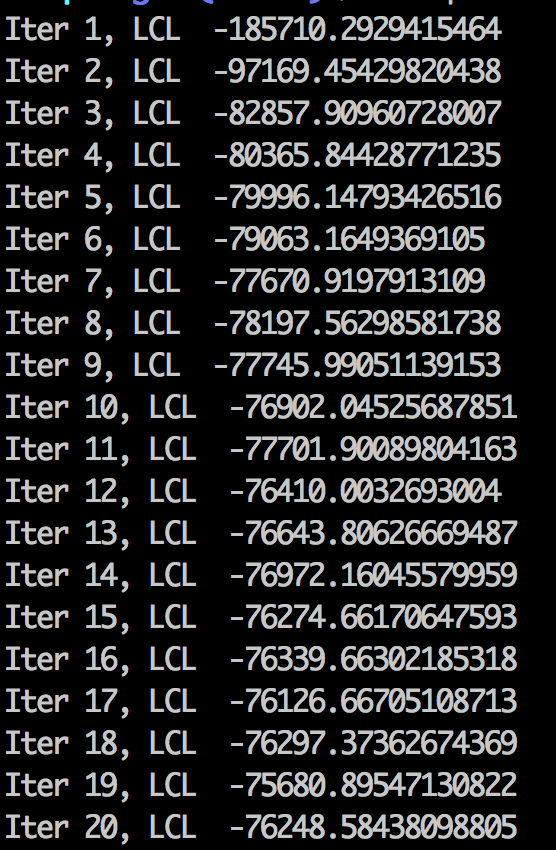
\includegraphics[width=6cm]{pic/q1.png}
\end{center}
\caption{LCL over iterations}
\end{figure}

\section{Question 2}

The accuracy curve of the 11 different parameters is:

\begin{figure}[h]
\begin{center}
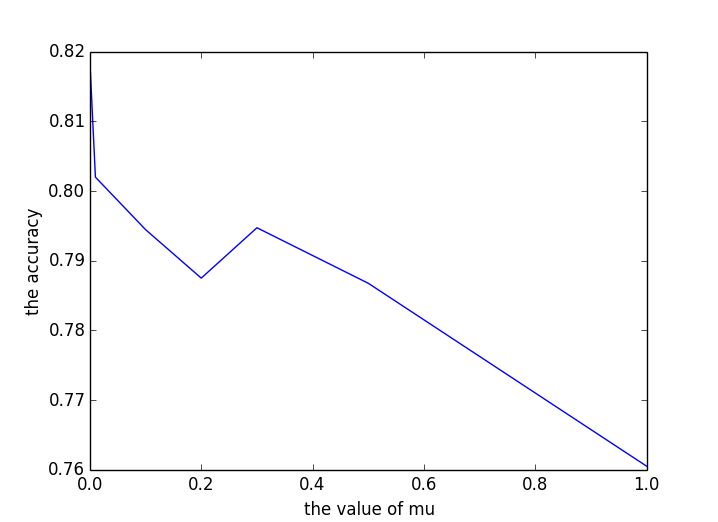
\includegraphics[width=10cm]{pic/q21.png}
\end{center}
\caption{Accruracy over mu, whole range}
\end{figure}

We could see the general trend of the performances is first arising with the x,
then decreasing. To see it in details, we can draw a figure in small range:

\begin{figure}[h]
\begin{center}
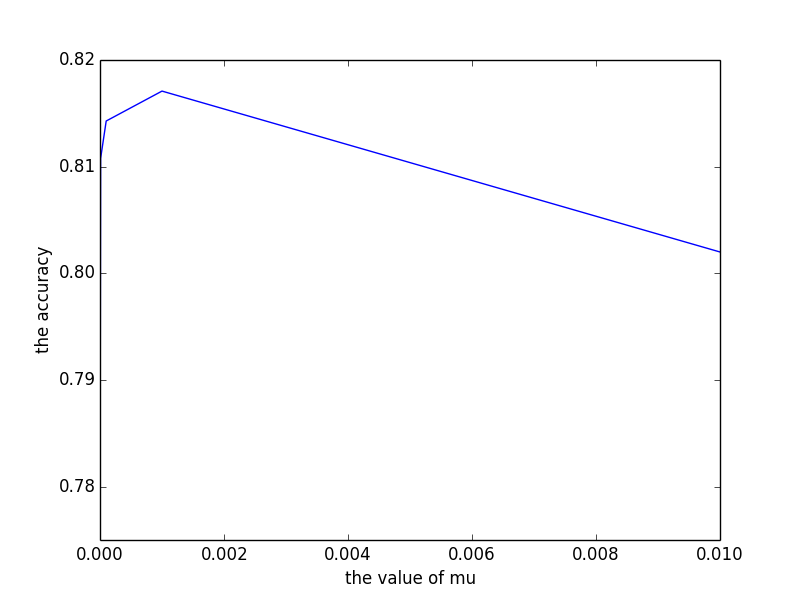
\includegraphics[width=10cm]{pic/q22.png}
\end{center}
\caption{Accuracy over mu, small range}
\end{figure}

We could find that the best point is when mu is 0.001. I think this result is
very reasonable. As we all know, the mu is used to do regularization. If the
mu is too small, then the model would be overfitting, which would lower the
performances. On the other hand, if mu is too big, then many parameters would
vanish towards zero, which would make the model too ``simple'', and also lower
the accuracy.



\section{Question 3}

The result is as follows, we could see that the best D is the $10^5$.

\begin{figure}[h]
\begin{center}
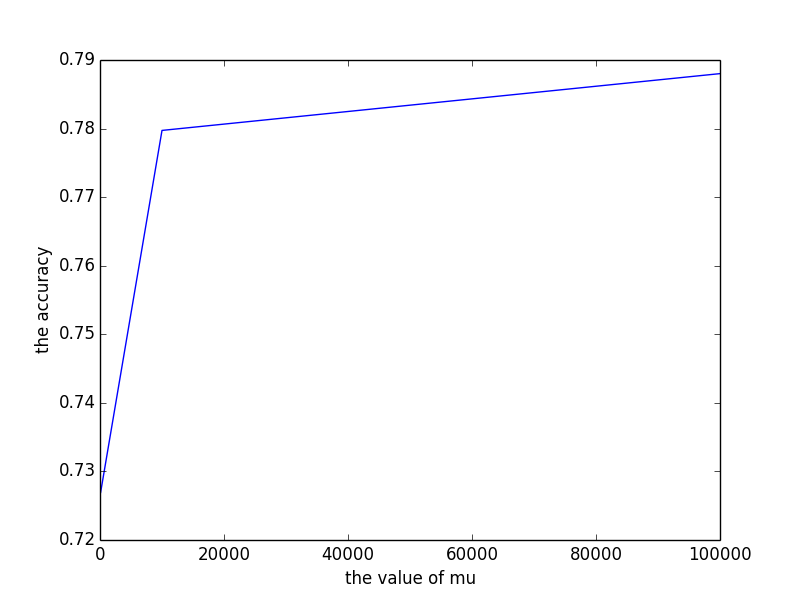
\includegraphics[width=10cm]{pic/q3.png}
\end{center}
\caption{Accuracy over D}
\end{figure}

Besides, we could see that the trend of the accuracy curve is very reasonable.
We could see that the accuracy is improving with the increasement of x. However,
the trend is becomming more and more slow. When x is small, the increasing of
feature space would bring much performances improvment. When x is big,
increasing the feature space would not be very effective. This is reasonable,
and proves that hash tricks is an reasonable way for large datasets.



\section{Question 4}

We can use different threshold and got different iterations. The specific result
is here:

First, threshold: 100, running time: 26.0865, accuracy: 0.670113

Second, threshold: 50, running time: 39.692, accuracy: 0.813421

Third, using SGD, running for 20 iters, time: 29.548, accuracy 0.812102

As we can see here, if we set the threshold to a very small value, then the
program would take more time to converge, and got a better performances.



\section{Question 5}

No, we can not guarantee that arriving to the same W and H everytime. This is
because for the matrix factorization task, we just random initilization and
then doing the updates in every iteration. What's more, the iteration number
was not sure to guarantee that the algorithm would converge to the same point.



\section{Question 6}

The (b) is not valid for DSGD, because it does not satisfy the requirements of
the strata for the DSGD algorithms. In the DSGD algorithms, the set of blocks,
the stratum, should not overlap. But in (b), the blocks are overlapped.



\section{Question 7}

The (d) strata should only achieve a suboptimal from the point of
view of parallelism. This is because in DSGD, we need to group the data. We should
repeat that untill all blocks are covered. Otherwise, we are not taking the whole
dataset. Therefore, losing a block of data would cause a suboptimal of the dataset from the point
of view of parallelism.



\section{Question 8}

I did not receive helps from others, and did not give direct helps to others.

\end{document}
